\section{Object reconstruction and event selection}
\label{event_sel}

The CMS offline event reconstruction uses the particle-flow (PF)
algorithm~\cite{CMS-PAS-PFT-10-002} to identify the physics objects as PF
muons, electrons, photons and hadrons which are used in this analysis.

\subsection{Muon reconstruction}

The muon candidates are reconstructed by matching compatible track segments
from the inner silicon tracker and the muon detectors~\cite{Chatrchyan:2012xi}.
They are required to be reconstructed within the pseudorapidity range of
$|\eta|< 2.4$ and have transverse momentum $p_{T} > 10$.
They are additionally required to be sufficiently isolated in a cone
$\Delta R\equiv\sqrt{\Delta\eta^{2}+\Delta\phi^{2}}<0.4$ around the
muon candidate. The $\Delta \beta$-corrected isolation:

$I_{rel}^{PF}=(p_{T}^{ch}+max(0,E_{T}^{\gamma}+E_{T}^{nh}-0.5*p_{T}^{chPU}))/p_{T}^{\mu}$

where $p_{T}^{ch}$ is the charged hadron transverse momenta sum,
$E_{T}^{\gamma}$ is the photon transverse energy sum, and $E_{T}^{nh}$
is the neutral hadron transverse energy sum. The term $p_{T}^{chPU}$ is the estimated
transverse momentum of charged particles from pileup in the $\Delta R < 0.4$ cone,
and the factor of 0.5 is used to estimate the neutral pileup from the charged component.
The relative muons isolation is required to be $I_{rel}^{PF}<0.25$.

%% \subsection{Electrons}
%% Electron candidates are reconstructed starting with an electromagnetic
%% calorimeter (ECAL) energy cluster which matches the momentum associated to a
%% track in the silicon tracker~\cite{Khachatryan:2015hwa}. The PF Electrons
%% have to be isolated with \pt greater than 10 GeV and to be within the ECAL
%% fiducial region of $|\eta|<1.4442$ or $1.566<|\eta|<2.5$.

%% The working point chosen for the PF muon (electron) candidates and the
%% corresponding isolation leads to an efficiency of 90\%(80-86\%), depending
%% on $p_T$ and $\eta$. MC simulated samples are corrected for differences
%% observed in reconstruction and isolation efficiency between data and MC
%% using the dilepton $Z$ boson reconstruction.

\subsection{Jet reconstruction}
Jets are reconstructed from PF candidates with the anti-$\kappa_{T}$
algorithm~\cite{Cacciari:2008gp} with a distance parameter of 0.4 after
rejecting the charged hadrons that are associated to pileup primary vertices.
Jets overlapping with the selected PF muons are not
considered further in the analysis. The selected jets with a minimum \pt
of 30 GeV and a maximum $|\eta|$ of 4.7 are corrected in energy in order to
account for the non-uniform detector response.

The PF jets are further required to fulfill the jet identification criteria.
Jets with $|\eta|$ less than 2.7 are required to contain at
least one charged PF candidate and have a non-zero charged energy fraction,
and a charged electromagnetic energy fraction less than 0.99. The
neutral and photon energy fraction must be less than 0.99. Jets in
the region $2.7<|\eta|<3.0$ are required to have a neutral electromagnetic
fraction of greater than 0.01 and neutral hadron fraction less than
0.98 while jets with pseudorapidity above 3.0 are required to have more
than 10 neutral particles and a neutral electromagnetic energy fraction
less than 0.9.

For reconstructed jets with $|\eta| < 2.4$, the combined secondary vertex b-tagging
algorithm (CSVv2)~\cite{Chatrchyan:2012jua} response is used to discriminate
against the $t\bar{t}$ background process events when defining the event
categories. The CSVv2 medium operating point is chosen as base line for this
analysis and corresponds to a b-tagging efficiency of $60-65\%$ while the
misidentification rate for light quarks such as $u$, $d$, $s$, and gluon jets
is approximately 1\%.

\subsection{Muon corrections}

TODO

\begin{itemize}
\item Muon ID and Isolation efficiency scale factors
\item HLT\_Iso(Tk)Mu24 efficiency scale factors
\item Rochester and Kalman Muon momentum corrections
\end{itemize}

\subsection{Jet and MET corrections}

TODO

\begin{itemize}
\item Jet energy scale corrections (propagated to MET)
\item Bad muon MET filters
\end{itemize}

\subsection{Event selection}

This analysis uses the lowest-\pt unprescaled single isolated muon trigger
path available during all included data taking periods.
These triggers require the event to have at least one isolated muon
candidate with \pt above 24 GeV, with no explicit restriction
on its pseudorapidity.

Proton-proton collisions events are selected by requiring at least
one valid reconstructed primary vertex (PV). The PV with the highest
scalar sum of the squared \pt of its associated tracks, of which
it must have at least 4, is considered as the PV of the hard interaction
in the a certain beams bunch crossing.

Offline event selection requires at least two opposite-charge muons
which pass the muon identification criteria mentioned previously.
The two highest-\pt selected muons with opposite charge are considered
as the \Htomm candidate pair.  At least one of these muons must have
\pt greater than 26 GeV, and be matched to a trigger muon with
$\Delta R < 0.1$.

\subsection{Object validation}

After applying all the selection cuts and scale factors, we validate the MC simulation
on data events where the candidate muon pair has an invariant mass greater than 60~GeV.

\begin{figure}[hbp]
  \centering
  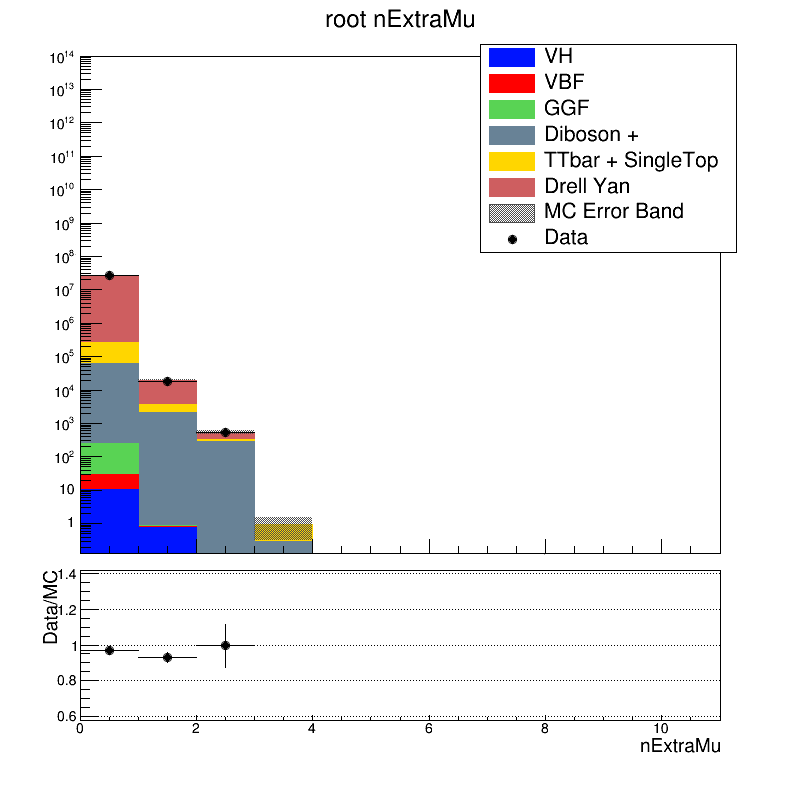
\includegraphics[width=0.32\linewidth]{figures/event_sel/nExtraMu_root.png}
  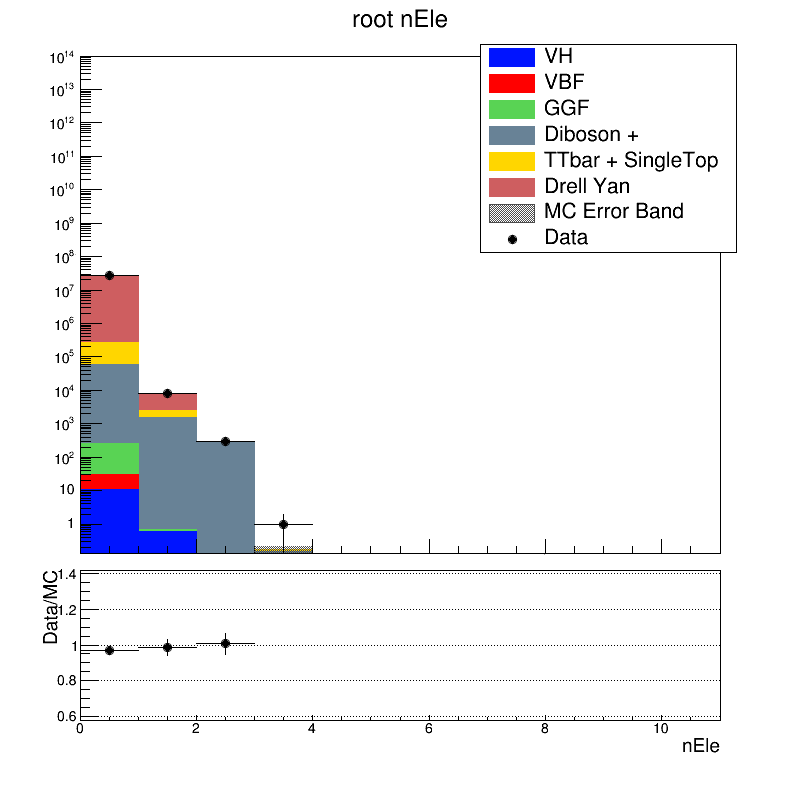
\includegraphics[width=0.32\linewidth]{figures/event_sel/nEle_root.png}
  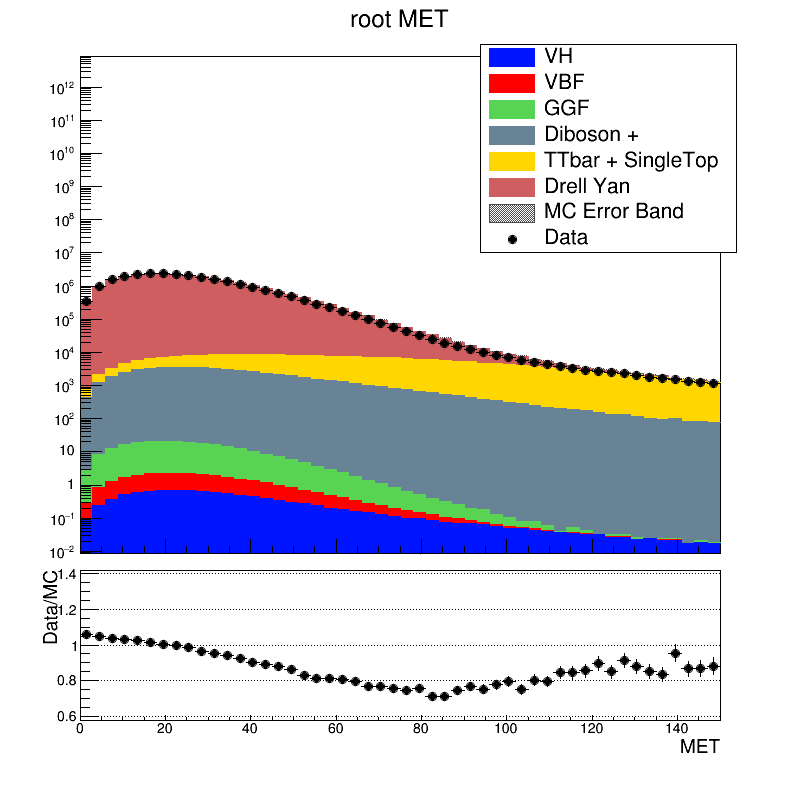
\includegraphics[width=0.32\linewidth]{figures/event_sel/MET_root.png}
  \caption
   {Validation of global event variables.}
  \label{fig:valid_evt}
\end{figure}

\begin{figure}[hbp]
  \centering
  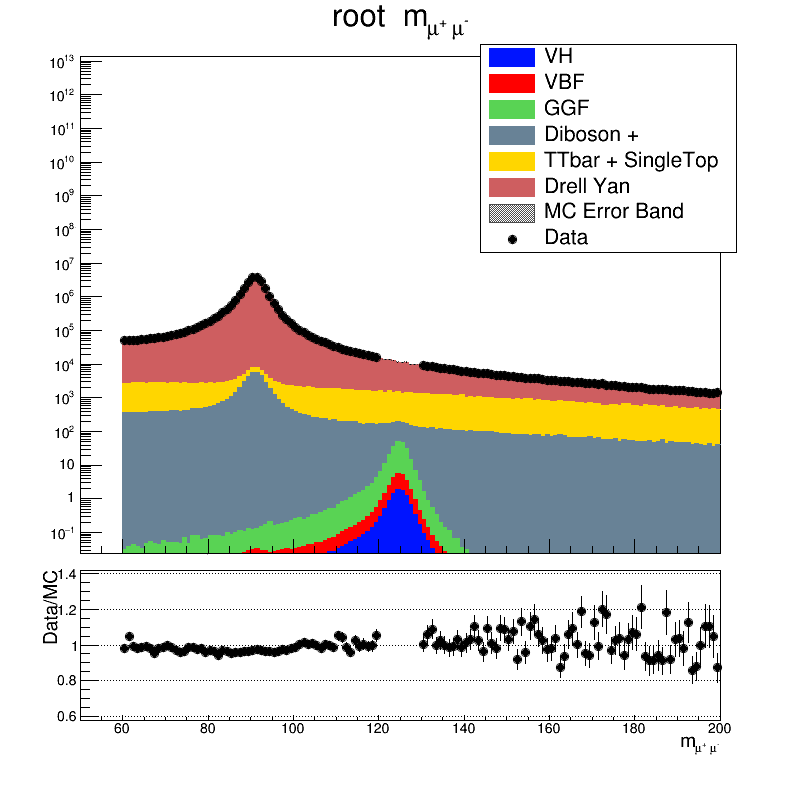
\includegraphics[width=0.32\linewidth]{figures/event_sel/dimu_mass_Roch_root.png}
  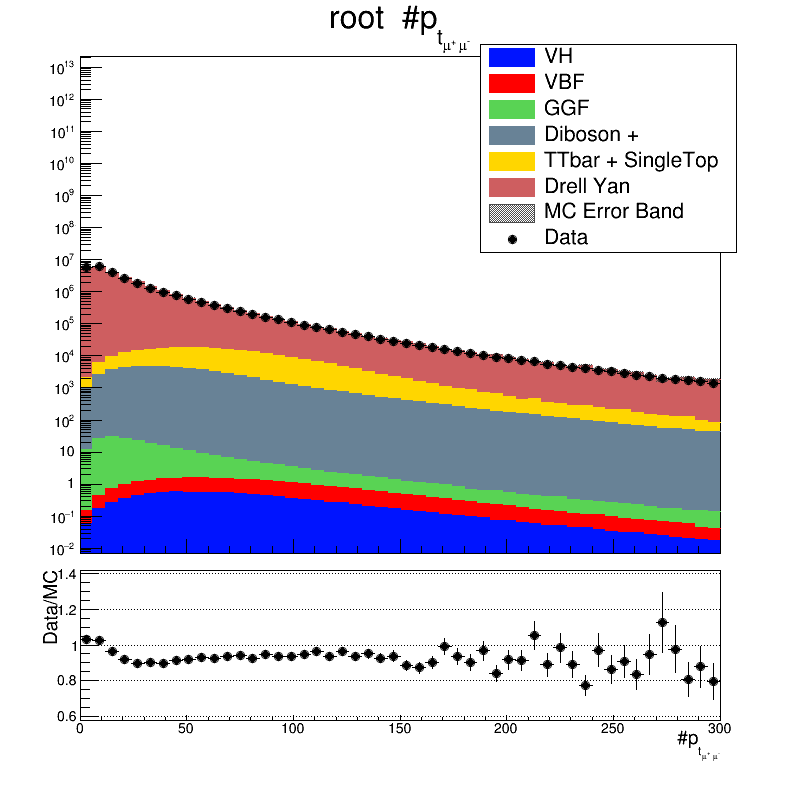
\includegraphics[width=0.32\linewidth]{figures/event_sel/dimu_pt_root.png}
  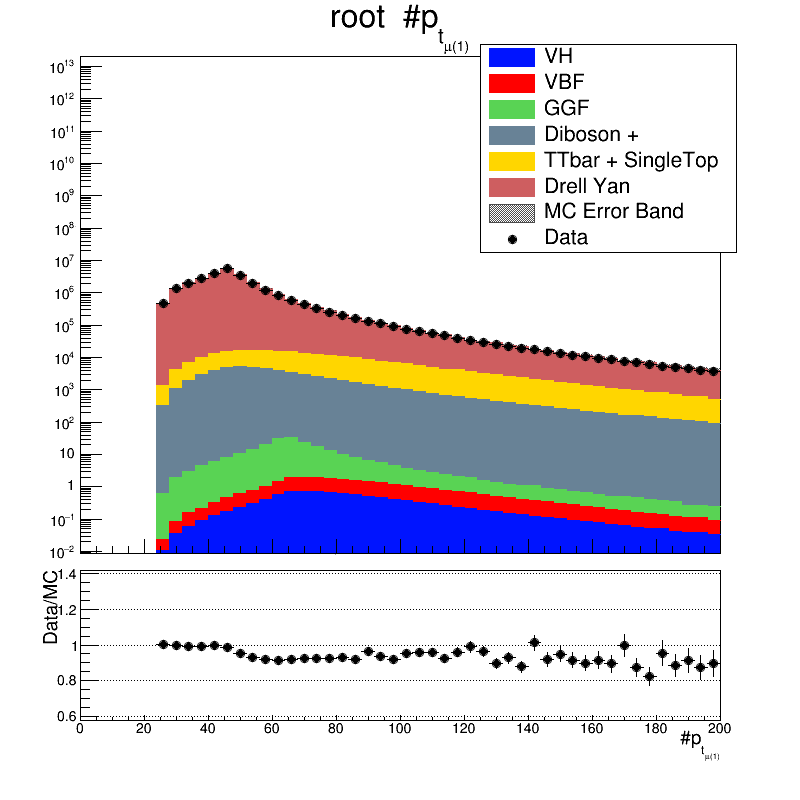
\includegraphics[width=0.32\linewidth]{figures/event_sel/mu1_pt_root.png}
  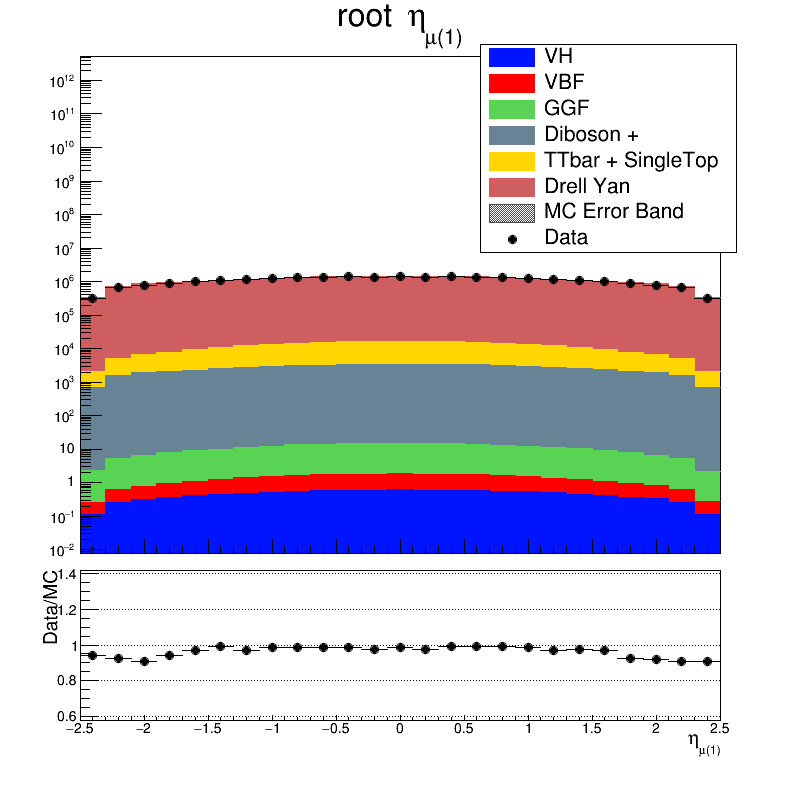
\includegraphics[width=0.32\linewidth]{figures/event_sel/mu1_eta_root.png}
  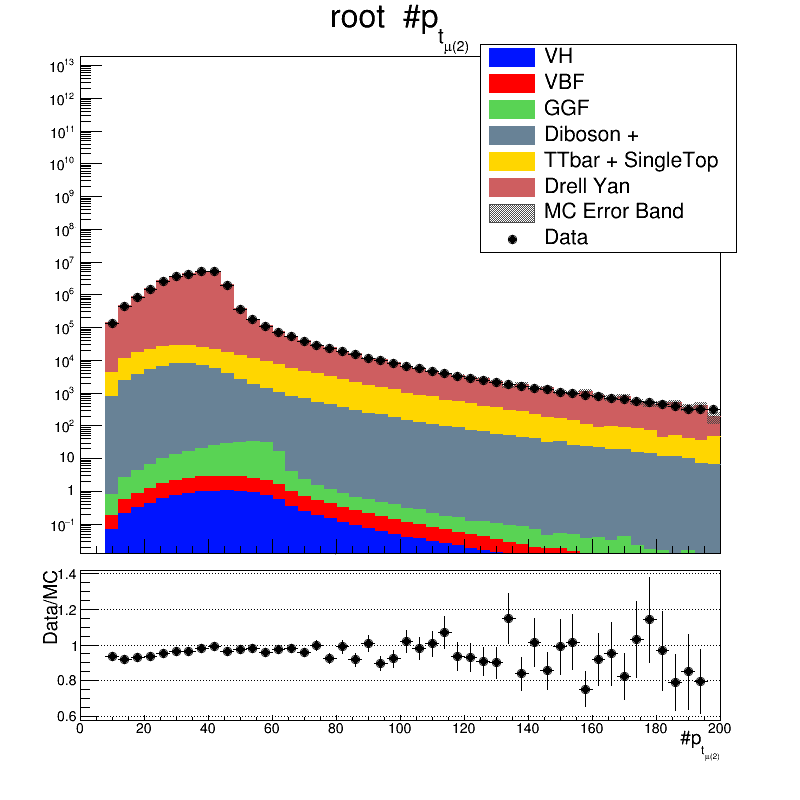
\includegraphics[width=0.32\linewidth]{figures/event_sel/mu2_pt_root.png}
  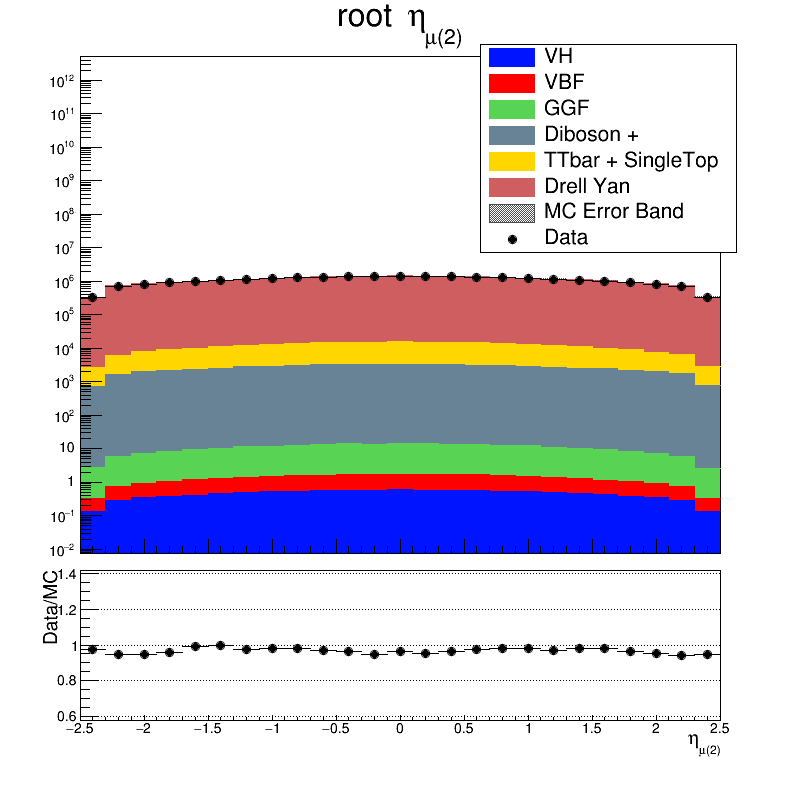
\includegraphics[width=0.32\linewidth]{figures/event_sel/mu2_eta_root.png}
  \caption
   {Validation of muon-related variables.}
  \label{fig:valid_muons}
\end{figure}

\begin{figure}[hbp]
  \centering
  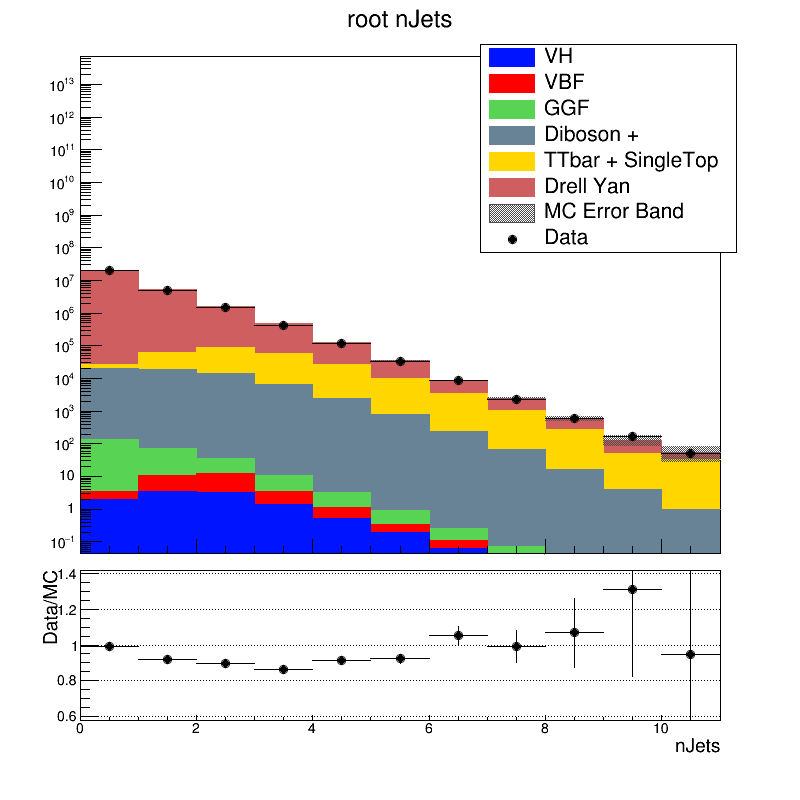
\includegraphics[width=0.32\linewidth]{figures/event_sel/nJets_root.png}
  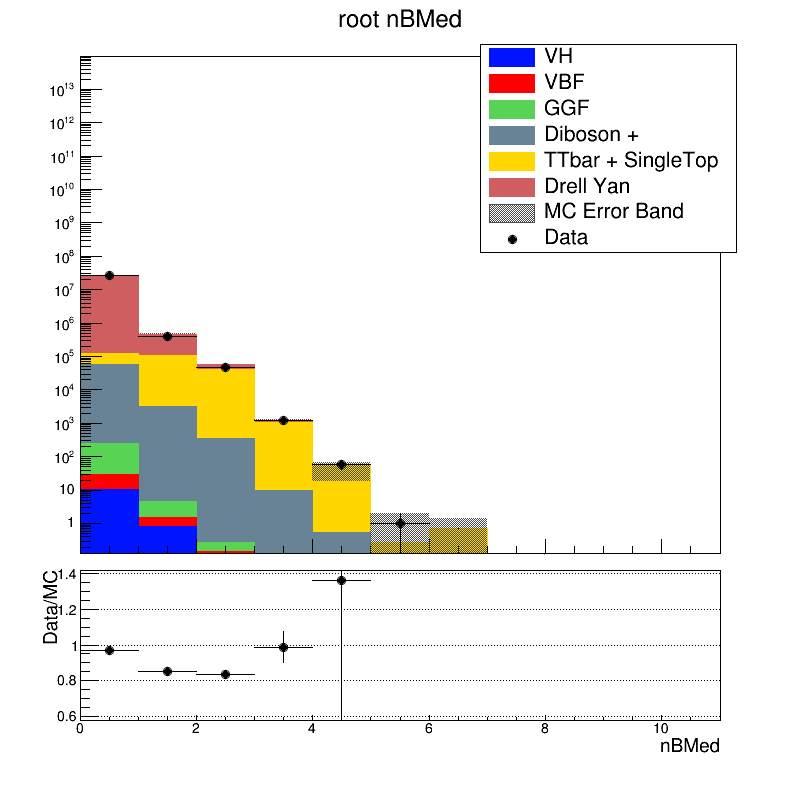
\includegraphics[width=0.32\linewidth]{figures/event_sel/nBMed_root.png}
  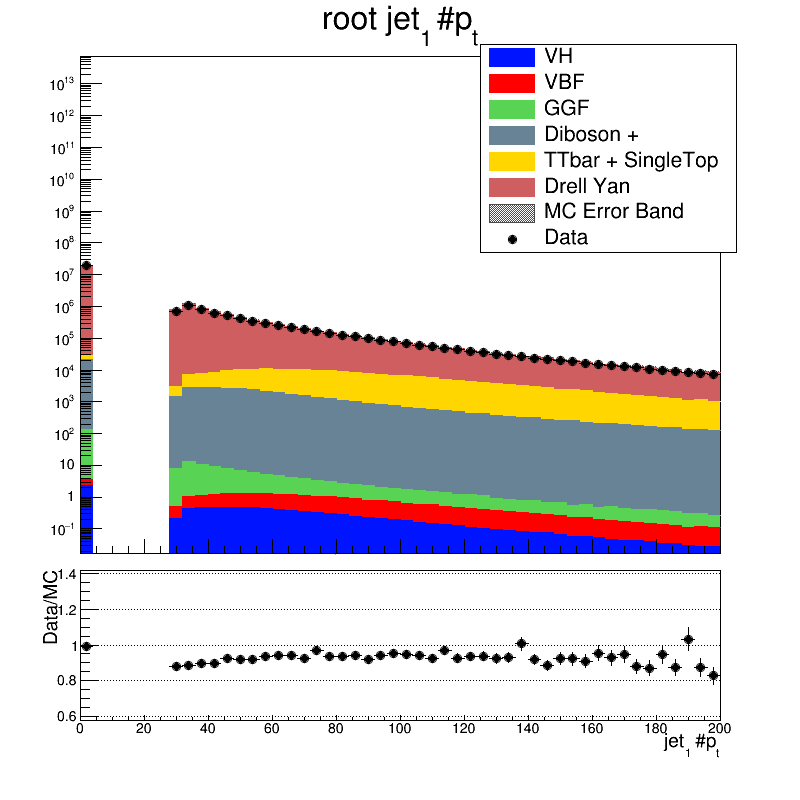
\includegraphics[width=0.32\linewidth]{figures/event_sel/jet1_pt_root.png}
  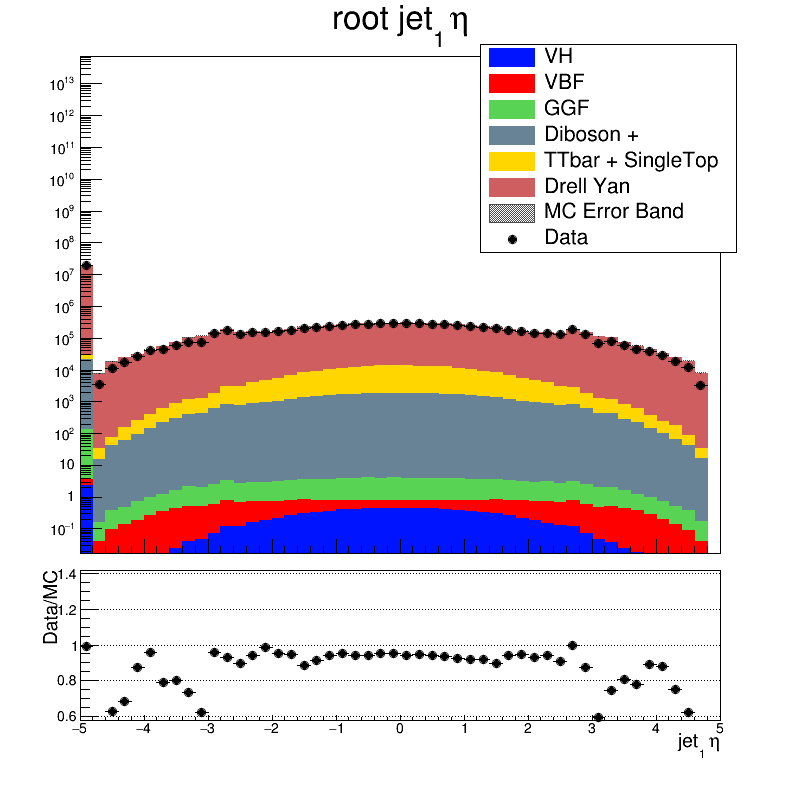
\includegraphics[width=0.32\linewidth]{figures/event_sel/jet1_eta_root.png}
  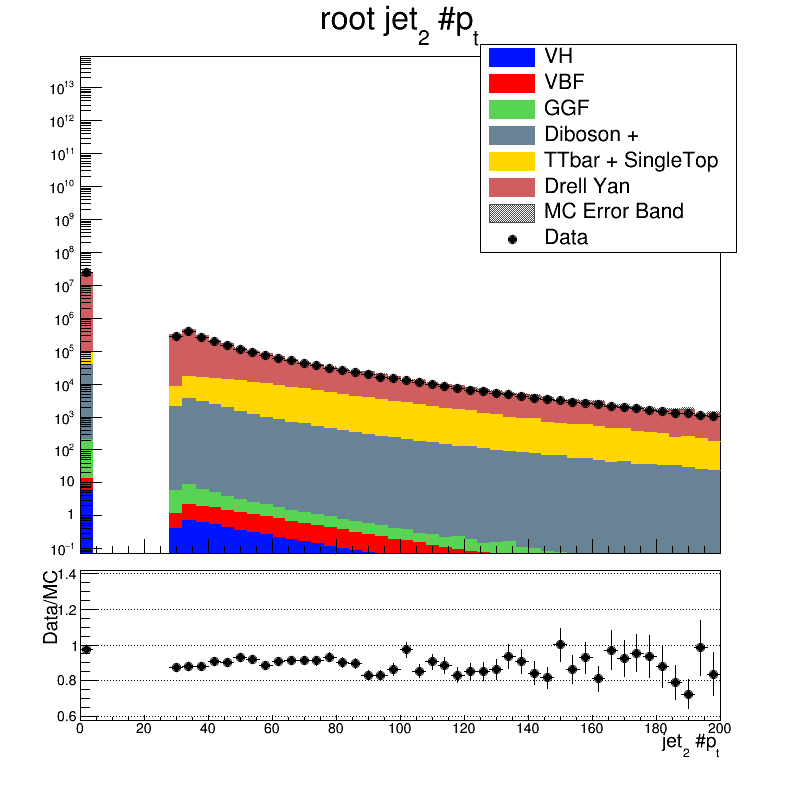
\includegraphics[width=0.32\linewidth]{figures/event_sel/jet2_pt_root.png}
  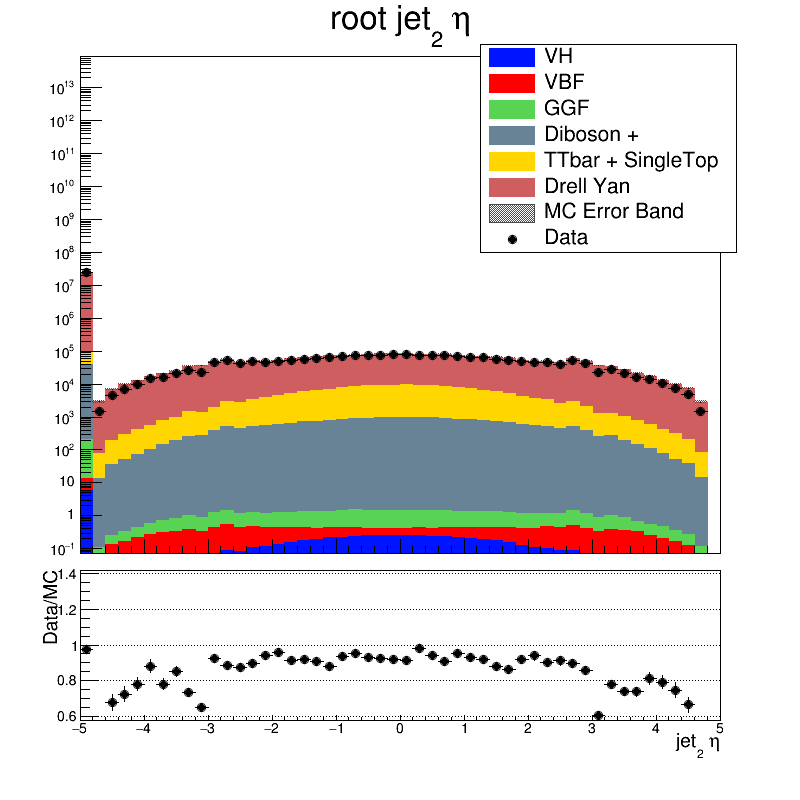
\includegraphics[width=0.32\linewidth]{figures/event_sel/jet2_eta_root.png}
  \caption
   {Validation of jet-related variables.}
  \label{fig:valid_jets}
\end{figure}



